\section{\probidx. \probname}

\begin{frame} % No title at first slide
	\sectiontitle{\probidx}{\probname}
	\sectionmeta{
		\texttt{number-theory, constructive}\\
		출제진 의도 -- \textbf{\color{acdiamond} Easy}
	}
	\begin{itemize}
		\item 제출 ?번, 정답 ?명 (정답률 ?.???\%)
		\item 처음 푼 사람: \textbf{???}, ?분
		\item 출제자: \texttt{gumyeol}
	\end{itemize}
\end{frame}

\begin{frame}{\textbf{\probidx}. \probname}
	\begin{itemize}
		\item 암석 관찰을 통해 제주도에 존재하는 욤암류 분석
		\item 아아 용암(A'a lava), 파호이호이 용암(Pāhoehoe lava)을 중점적으로 비교
		\item 자연탐사에서 방문한 금능해변과 수월봉, 한라산 그리고 곶자왈에 대해 연구
	\end{itemize}
\end{frame}


\begin{frame}{\textbf{\probidx}. \probname}
	\begin{itemize}
		\vspace{1em}
		\item 금능해변

		      \vspace{1em}
		      \begin{minipage}{.25\textwidth}
			      \begin{center}
				      \begin{figure}[bh]
					      \centering
					      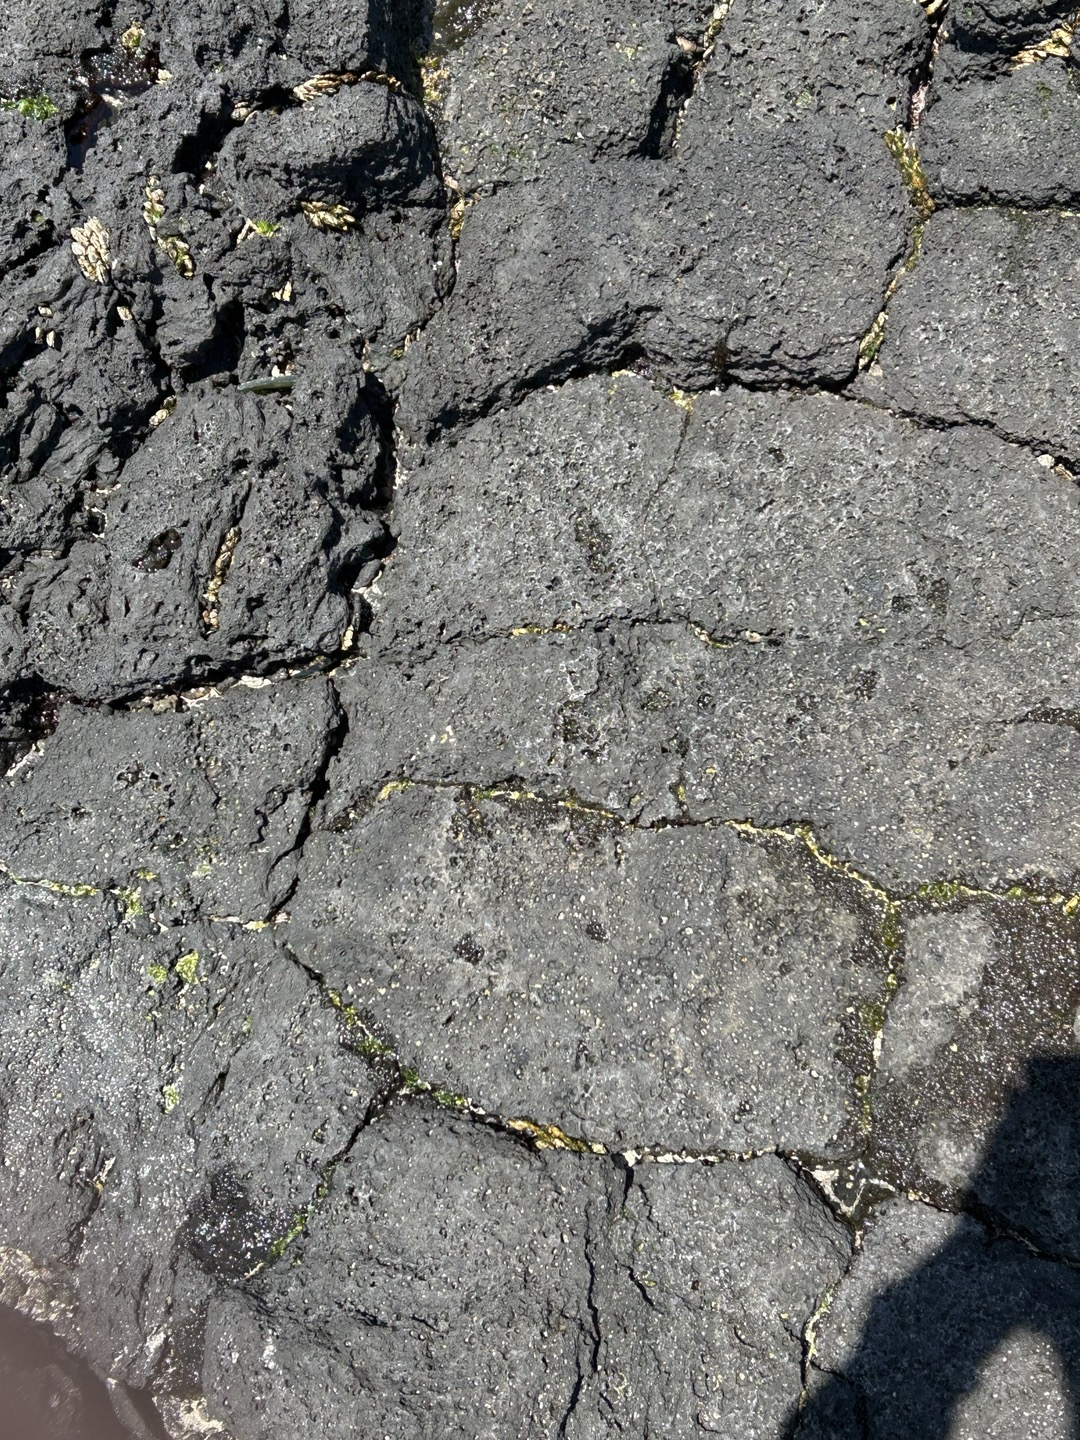
\includegraphics[width=\linewidth]{gn_a.jpeg}
					      \caption{Fig. 1: 아아 용암}
				      \end{figure}
			      \end{center}
		      \end{minipage}
		      \begin{minipage}{.1\textwidth}
		      \end{minipage}
		      \begin{minipage}{.25\textwidth}
			      \begin{center}
				      \begin{figure}[bh]
					      \centering
					      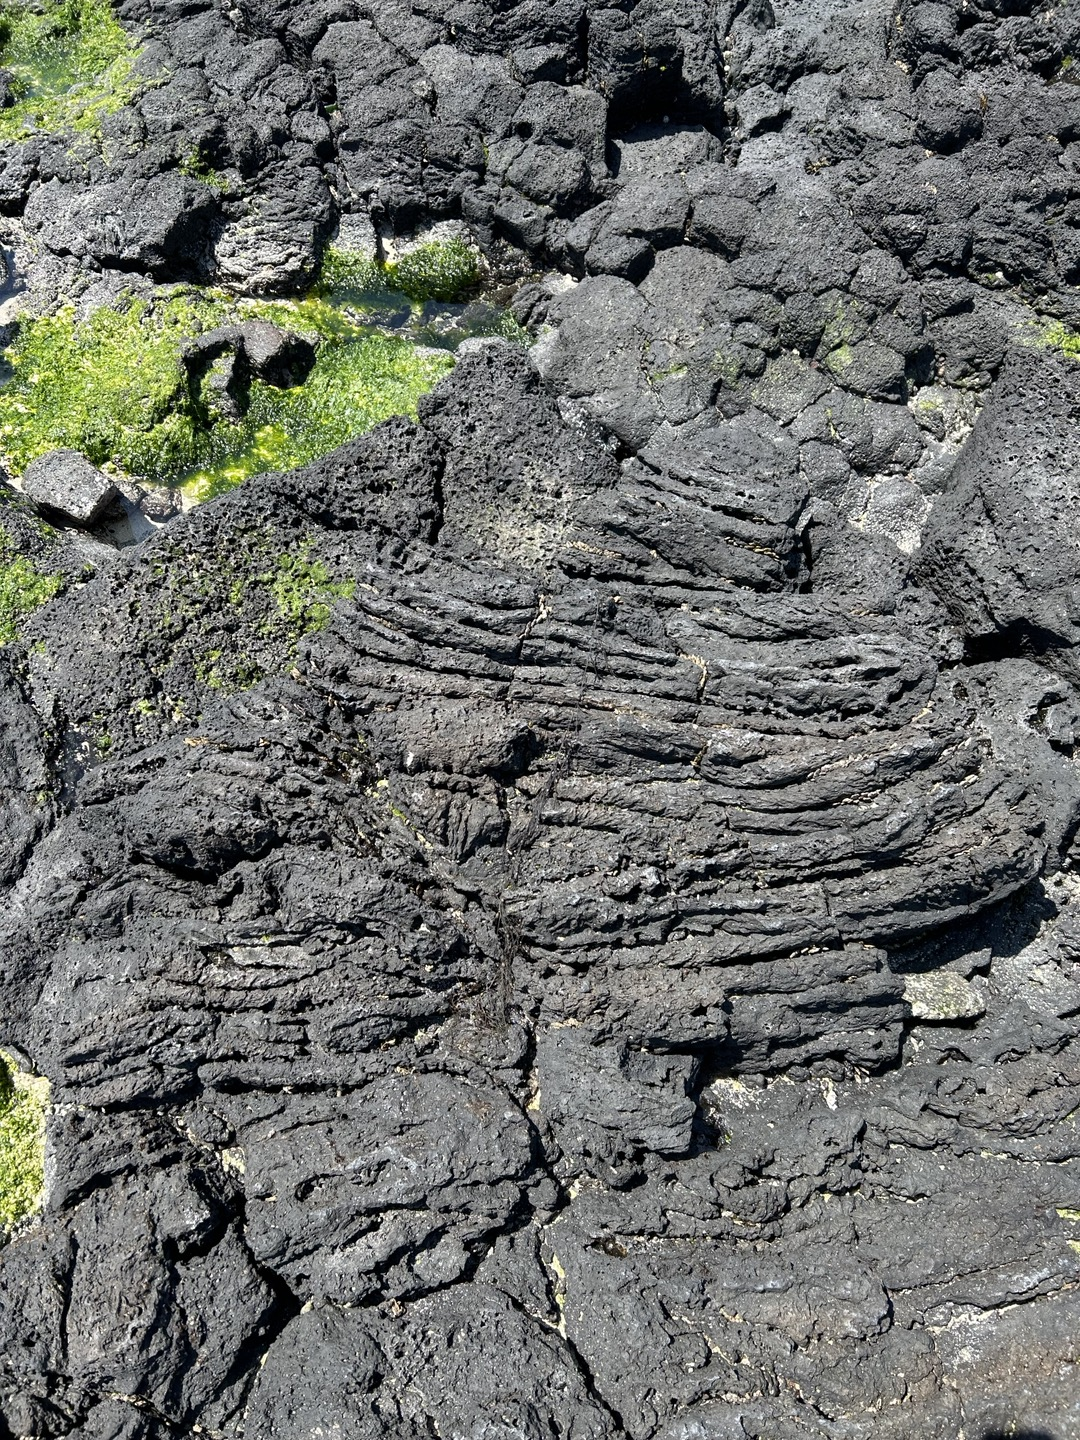
\includegraphics[width=\linewidth]{gn_p.jpeg}
					      \caption{Fig. 2: 파호이호이 용암의 새끼줄 구조}
				      \end{figure}
			      \end{center}
		      \end{minipage}
	\end{itemize}
\end{frame}